\documentclass[../index.tex]{subfiles}
\begin{document}
    \subsection{Zadania}

    \textbf{Zadanie 8.} Dla jakich $n \in \mathbb{N}$ wszystkie elementy zbioru $\{0,1,2\}^n$ można ułożyć
    \begin{itemize}
        \item[(a)] w ciąg;
        \item[(b)] w cykl;
    \end{itemize}
    w taki sposób, aby każde dwa sąsiednie wyrazy różniły się dokładnie na jednej pozycji i to dokładnie o 1?

    \textbf{Zadanie 9.} Układamy $n$ identycznych tomów encyklopedii na półce — mogą stać pionowo lub poziomo, przy czym poziome tomy mogą leżeć jeden na drugim tworząc stosy. Ile jest różnych sposobów ustawienia tomów?

    Przykładowo dla $n=2$ poprawna odpowiedź to 5:
    \begin{center}
        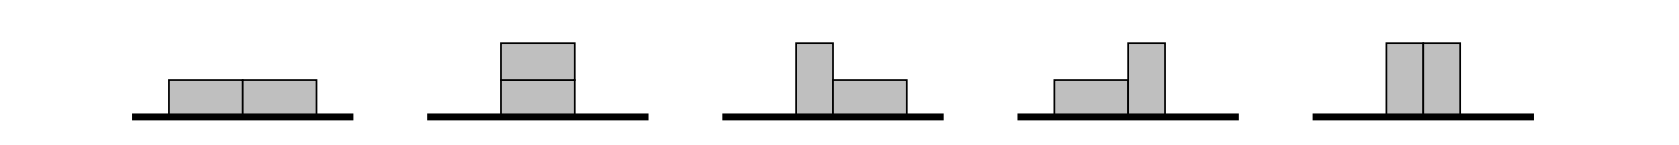
\includegraphics[width=0.7\textwidth]{books.png}
    \end{center}

    \textbf{Zadanie 10.} Niech $B_n$ oznacza \textit{pełne drzewo binarne} o wysokości $n$. Ciąg $(B_n)$ jest zdefiniowany rekurencyjnie następująco: $B_0$ składa się wyłącznie z korzenia, a dla $n \geq 1$ korzeń $B_n$ ma dwóch synów, z których każdy jest korzeniem $B_{n-1}$.

    \begin{itemize}
        \item[(a)] Wyznacz sumę głębokości wszystkich węzłów w $B_n$.
        \item[(b)] Wyznacz sumę długości wszystkich ścieżek w $B_n$.
    \end{itemize}

    Na rysunku $B_3$ z zaznaczoną ścieżką o długości 3.

    \begin{center}
        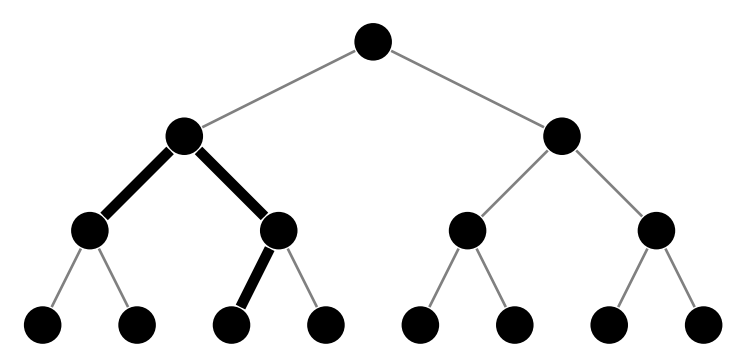
\includegraphics[width=0.5\textwidth]{binary_tree.png}
    \end{center}

    \textbf{Zadanie 11.} Niech $\langle x_n \rangle_{n \geq 0}$ będzie ciągiem zadanym przez $x_0 = 1$, $x_1 = 2025$ oraz
    \[
    x_{n+2} = 4050 x_{n+1} - (2025^2 + 1) x_n \quad \text{dla } n \geq 0.
    \]
    Rozstrzygnij, czy wszystkie wyrazy ciągu $\langle x_n \rangle$ są dodatnie.

\end{document}
